\documentclass[../main.tex]{subfiles}

\begin{document}

\chapter{June $20^{th} / 2025$}
\label{ch:tufte-design}

\section{MASCARA: Coexpression analysis in data from designed experiments}\cite{WHITE2025100052}

\hrulefill

\textbf{MASCARA (Mixed-dAtatype State-space model for analyzing clinicAl tRajectories)}: Probabilistic framework designed to model longitudinal dynamics of multiple variables of mixed data types (e.g., continuous, categorical, count). The core of MASCARA is a State-Space Model (SSM), which posits that observed data are generated from an unobserved (latent) state that evolves over time.

\vspace{0.3cm}

\textbf{Differential Expression Analysis (DE)}: Determines which features are expressed differently between $2$ or more experimental conditions.

\vspace{0.3cm}

\textbf{Coexpression Analysis (CoE)}: Aims at discovering features that are part of an already partially characterized pathway of interest (POI). the expression profiles of known features of POI (baits) are used to detect novel pathways members with similar expressuin or accumulation patterns (targets).

\begin{center}
    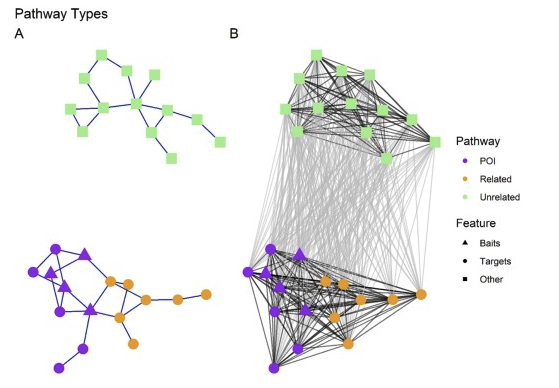
\includegraphics[width=6.5cm]{files/images/pathwy_types.png}
\end{center}

\section{Mathematical Framework}
SSM consists of $2$ primary components: state equation and observation equation

\subsection{State Equation (Transition Model)}
The evolution of the system is captured by a low-dimensional latent state vector $\mathbf{z}_t \in \mathbb{R}^L$ at each time point $t$. MASCARA models this evolution as a linear Gaussian process, such as a random walk.
\begin{equation}
    \mathbf{z}_t | \mathbf{z}_{t-1} \sim \mathcal{N}(\mathbf{A} \mathbf{z}_{t-1}, \mathbf{Q})
\end{equation}
where $\mathbf{A}$ is the transition matrix and $\mathbf{Q}$ is the process noise covariance matrix. For a simple random walk, $\mathbf{A}$ is the identity matrix.

\subsection{Observation Equation (Emission Model)}
The link between the latent state $\mathbf{z}_t$ and the observed variable $y_{j,t}$ is modeled using a generalized linear model framework [2]. For categorical variables, which are most relevant to the ClinVar analysis, a multinomial logistic regression model is used.

Probability of observing category $k$ for $j$-th variable at time $t$:
\begin{equation}
    P(y_{j,t} = k | \mathbf{z}_t) = \text{softmax}(\mathbf{W}_j \mathbf{z}_t + \mathbf{b}_j)_k
\end{equation}
For a vector $\mathbf{x}$:
\begin{equation}
    \text{softmax}(\mathbf{x})_k = \frac{\exp(\mathbf{x}_k)}{\sum_{l=1}^{K} \exp(\mathbf{x}_l)}
\end{equation}
$\mathbf{W}_j$ and $\mathbf{b}_j$ learned during model fitting

\subsection{Model Inference} 
The model parameters and latent states are estimated using \textbf{Stochastic Variational Inference (SVI)} makes method scalable to large datasets. PyTorch SVI framework.



\end{document}